%==============================================================================
%  Architecture and Preprocessing Choices under Dataset Shift in Single-Channel
%  EEG Sleep Staging: A Controlled Evaluation on Sleep-EDF and SHHS1
%
%  English manuscript. Journal-neutral single-column preprint format.
%  Build:  pdflatex -> bibtex -> pdflatex -> pdflatex
%==============================================================================
\documentclass[11pt,a4paper]{article}

\usepackage[no-math]{fontspec}\setmainfont{Times New Roman}


\usepackage{newtxmath}   % Times-like text + math (journal convention)
\usepackage{microtype}
\usepackage{geometry}
\usepackage{amsmath}
\usepackage{graphicx}
\usepackage{booktabs}
\usepackage{tabularx}
\usepackage{array}
\usepackage{multirow}
\usepackage{caption}
\usepackage{subcaption}
\usepackage[section]{placeins}
\usepackage{xcolor}
\usepackage{enumitem}
\usepackage{xurl}
\usepackage{xr-hyper}
\usepackage{hyperref}
\externaldocument[SM-]{../paper_en/supplement}[SleepTCN_Supplement_EN.pdf]
\usepackage{fancyhdr}
\usepackage{authblk}               % structured author / affiliation block
\usepackage{titlesec}
\usepackage{abstract}

\geometry{top=2.4cm,bottom=2.4cm,left=2.3cm,right=2.3cm}
\setlength{\parindent}{1.1em}
\setlength{\parskip}{0.2em}\setlength{\emergencystretch}{2em}
\setlist{nosep,leftmargin=1.6em}
\captionsetup{font=small,labelfont=bf,labelsep=period}
\renewcommand{\arraystretch}{1.15}
\newcolumntype{Y}{>{\raggedright\arraybackslash}X}
\newcolumntype{C}[1]{>{\centering\arraybackslash}p{#1}}

% ---- section headings: journal-style, not oversized -------------------------
\titleformat{\section}{\normalfont\large\bfseries}{\thesection.}{0.6em}{}
\titleformat{\subsection}{\normalfont\normalsize\bfseries}{\thesubsection.}{0.6em}{}
\titleformat{\subsubsection}{\normalfont\normalsize\itshape}{\thesubsubsection.}{0.6em}{}
\titlespacing*{\section}{0pt}{1.5ex plus .3ex}{0.8ex}
\titlespacing*{\subsection}{0pt}{1.2ex plus .3ex}{0.6ex}

% ---- author block formatting (authblk) --------------------------------------
\renewcommand\Authfont{\normalsize}
\renewcommand\Affilfont{\small\itshape}
\setlength{\affilsep}{0.7em}
\renewcommand\Authand{ và }\renewcommand\Authands{ và }         % no "and" before the last author
\renewcommand\Authsep{, }

% ---- abstract block ---------------------------------------------------------
\renewcommand{\abstractnamefont}{\normalfont\bfseries}
\renewcommand{\abstracttextfont}{\normalfont\small}
\setlength{\absleftindent}{0.6cm}
\setlength{\absrightindent}{0.6cm}

\definecolor{linkblue}{RGB}{18,82,148}
\hypersetup{
  colorlinks=true,
  linkcolor=linkblue,
  citecolor=linkblue,
  urlcolor=linkblue,
  pdftitle={Lựa chọn kiến trúc và tiền xử lý khi chuyển bộ dữ liệu trong phân giai đoạn giấc ngủ từ EEG đơn kênh},
  pdfauthor={Ngô Nhật Quân; Phạm Thái Sơn; Tri Nguyen Ho Duy; Tri Nguyen},
  pdfkeywords={sleep staging; single-channel EEG; temporal convolutional network; preprocessing; domain shift; paired evaluation}
}

\pagestyle{fancy}
\fancyhf{}
\fancyhead[L]{\small\itshape Ngô và cộng sự}
\fancyhead[R]{\small\itshape Phân giai đoạn giấc ngủ khi chuyển bộ dữ liệu}
\fancyfoot[C]{\thepage}
\setlength{\headheight}{14pt}
\renewcommand{\headrulewidth}{0.4pt}

\newcommand{\mf}{\ensuremath{\mathrm{macro\text{-}F1}}}
\newcommand{\ci}{\ensuremath{\mathrm{CI}_{95\%}}}
\newcommand{\dsign}{\ensuremath{\Delta_{\mathrm{sign}}}}

%==============================================================================
\begin{document}
\renewcommand{\abstractname}{Tóm tắt}
\renewcommand{\refname}{Tài liệu tham khảo}
\renewcommand{\figurename}{Hình}
\renewcommand{\tablename}{Bảng}

%------------------------------------------------------------------ front matter
\title{\bfseries\LARGE Lựa chọn kiến trúc và tiền xử lý khi chuyển bộ dữ liệu trong phân giai đoạn giấc ngủ từ EEG đơn kênh\\[0.2em]\Large Đánh giá có kiểm soát trên Sleep-EDF và SHHS1}
\author[a,$\ast$]{Ngô Nhật Quân}
\author[a]{Phạm Thái Sơn}
\author[a]{Tri Nguyen Ho Duy}
\author[a]{Tri Nguyen}
\affil[a]{Khoa Hệ thống Thông tin, Trường Đại học Công nghệ Thông tin,\protect\\
Đại học Quốc gia Thành phố Hồ Chí Minh,\protect\\
Khu phố 34, phường Linh Xuân, Thành phố Hồ Chí Minh, Việt Nam}

\date{\small Bản dịch tiếng Việt để đọc đối chiếu với bản thảo BSPC}

\maketitle
\thispagestyle{empty}

\vspace{-1.0em}
\begin{center}
\small
Ngô Nhật Quân: \texttt{23521258@gm.uit.edu.vn} $^{\ast}$(Tác giả liên hệ) \\[0.2em]
Phạm Thái Sơn: \texttt{23521361@gm.uit.edu.vn} \\[0.2em]
Tri Nguyen Ho Duy: \texttt{trinhd@uit.edu.vn} \\[0.2em]
Tri Nguyen: \texttt{tringuyen@uit.edu.vn}
\end{center}

\vspace{0.4em}

\vspace{-0.2em}

\begin{abstract}
\noindent
\textbf{Bối cảnh.} Lựa chọn mô hình và tiền xử lý có thể thay đổi độ chính xác phân giai đoạn giấc ngủ, chi phí tính toán và sai số khi chuyển giữa các quần thể nghiên cứu.

\noindent
\textbf{Phương pháp.} Sáu cấu hình được so sánh trên 78 đối tượng Sleep-EDF với cùng phép chia 10 fold, phân tích bootstrap bắt cặp và Wilcoxon--Holm. Đánh giá chuyển miền chính sử dụng 180 người tham gia Sleep Heart Health Study Visit 1 (SHHS1), không cập nhật trọng số. Chuẩn hóa theo bản ghi có tính transductive, tức sử dụng dữ liệu bản ghi đích đang được suy luận. Các can thiệp bắt cặp gồm ADAST ở ngân sách nhỏ và toàn nguồn.

\noindent
\textbf{Kết quả.} Cấu hình mạng dư một chiều (ResNet-1D) kết hợp mạng tích chập thời gian (TCN) với đổi thang biên độ cố định (E3) đạt \mf\ gộp 0.7904 trên Sleep-EDF, cao hơn cấu hình tương ứng chuẩn hóa theo bản ghi (E6) 0.0213 (\ci\ $[0.0122,0.0307]$; Holm $p=0.0012$). Seed thứ hai giữ nguyên chiều chênh lệch nhưng không còn đạt ý nghĩa thống kê sau hiệu chỉnh Holm. E3 đạt tốc độ truyền xuôi gấp $3.76\times$ đối chứng tích chập kết hợp bộ nhớ dài ngắn hạn hai chiều (CNN--BiLSTM), với số tham số gấp $4.37\times$. Trên SHHS1, E3 cải thiện \mf\ trung bình theo đối tượng so với đối chứng 0.0412 (\ci\ $[0.0314,0.0512]$). Các so sánh bổ sung trên cùng quần thể cho kết quả tốt hơn với E4 chỉ lọc thông dải so với E3 ở cả hai seed: chênh lệch 0.0131 (seed 42, \ci\ $[0.0111,0.0153]$) và 0.0098 (seed 123, \ci\ $[0.0073,0.0125]$). Cả hai quy trình chính đều phân loại nhầm hơn 72\% epoch N3 (ngủ sâu) thành N2; độ thu hồi N3 của E3 là 0.2582. ADAST toàn nguồn tăng \mf\ trung bình theo người 0.0445 (\ci\ $[0.0352,0.0539]$) so với đối chứng tương ứng; độ thu hồi N3 tăng 0.2432 lên 0.6111, nhưng F1 N1/N2/REM giảm.

\noindent
\textbf{Kết luận.} E3 kết hợp tốc độ tính toán nhanh hơn với kết quả chuyển quần thể tổng hợp tốt hơn đối chứng; E4 chỉ lọc thông dải đạt điểm SHHS1 cao hơn. Nhầm N3 thành N2 là sai số chủ đạo khi nhận diện ngủ sâu. Các kết quả này ủng hộ đánh giá đồng thời thiết kế mô hình, tiền xử lý và hiệu năng từng giai đoạn.
\end{abstract}

\vspace{0.3em}
\noindent\textbf{Từ khóa:} phân giai đoạn giấc ngủ; EEG đơn kênh; mạng tích chập thời gian; tiền xử lý; dịch chuyển miền; đánh giá bắt cặp.

\vspace{0.3em}


%==============================================================================
\clearpage
\section{Giới thiệu}

Phân giai đoạn giấc ngủ gán một trong năm nhãn W, N1, N2, N3 và REM cho mỗi đoạn tín hiệu (epoch) dài 30\,giây của bản ghi đa ký giấc ngủ. Chấm thủ công tốn thời gian, đòi hỏi người được đào tạo chuyên môn và vẫn có bất đồng giữa những người chấm; trong chương trình đánh giá độ tin cậy giữa người chấm của Viện Hàn lâm Y học Giấc ngủ Hoa Kỳ, N1 có mức đồng thuận thấp nhất trong các giai đoạn~\cite{rosenberg2013aasm}. Vì vậy, hệ thống tự động không thể chỉ được đánh giá bằng độ chính xác tổng thể, vốn chịu ảnh hưởng lớn của các giai đoạn xuất hiện nhiều nhất, mà còn cần các chỉ số cân bằng giữa các lớp, độ ổn định giữa các cá nhân và hành vi khi thiết bị ghi, cấu hình điện cực hoặc quần thể thay đổi.

Khó đánh giá tiến bộ của lĩnh vực chỉ qua các bảng kết quả đã công bố. Các nghiên cứu đồng thời khác nhau về phiên bản dữ liệu, cách chia theo đối tượng, quy tắc cắt bớt đoạn thức, lọc, chuẩn hóa, độ dài chuỗi và quy tắc chọn mô hình. Vì vậy, khó tách ảnh hưởng của kiến trúc khỏi những khác biệt khác trong quy trình giữa các nghiên cứu. Trong phát triển thực tế, các câu hỏi cần quan tâm là lựa chọn nào trong quy trình giúp dự đoán tốt hơn, chi phí tính toán tương ứng là bao nhiêu và lợi ích có được duy trì trên quần thể khác hay không. Để trả lời, cần dùng chung các phân hoạch đánh giá và mô tả rõ những gì thay đổi giữa các cấu hình, bao gồm cả quy trình huấn luyện.

Chúng tôi dùng ZleepAnlystNet~\cite{jadhav2024zleepanlystnet}, một mô hình đơn kênh hai giai đoạn kết hợp một nhóm bộ mã hóa tích chập chuyên biệt theo lớp với BiLSTM, làm đối chứng nội bộ. E1 thay cấu hình BiLSTM bằng mạng tích chập thời gian (TCN)~\cite{bai2018tcn}, dùng lại bộ mã hóa và đặc trưng đã lưu nhưng thay thiết lập huấn luyện mô hình chuỗi. E2 thay gói đặc trưng/ngữ cảnh hiện tại, trước và sau (C/P/N) 75 chiều của E1 bằng bộ mã hóa dư 128 chiều chỉ nhận epoch hiện tại~\cite{he2016resnet}, đồng thời thay cách huấn luyện và lựa chọn bộ mã hóa. Đây là so sánh giữa các cấu hình được xác định cụ thể, không phải phép đo tác động riêng của kiến trúc. Sau đó, các đối chiếu tiền xử lý khảo sát phép lọc và cách xử lý biên độ trong cùng mô hình ResNet-1D--TCN và cùng cấu hình huấn luyện.

Lựa chọn mô hình và cách xử lý tín hiệu có thể làm thay đổi cả chất lượng dự đoán lẫn chi phí tính toán. Tuy nhiên, kết quả tốt trên một bộ dữ liệu có thể thay đổi trên bộ dữ liệu khác. Từ đó, nghiên cứu đặt ra ba câu hỏi:
\begin{enumerate}[label=(\roman*)]
\item Các cấu hình mô hình được khảo sát khác nhau như thế nào về khả năng phân loại các giai đoạn giấc ngủ và nguồn lực tính toán cần sử dụng?
\item Với cùng kiến trúc mô hình và thiết lập huấn luyện, việc lọc tín hiệu và lựa chọn cách chuẩn hóa biên độ ảnh hưởng như thế nào đến kết quả phân loại?
\item Khi áp dụng trên dữ liệu của một nhóm người khác mà không cập nhật trọng số, cấu hình nào hoạt động tốt hơn và những giai đoạn giấc ngủ nào vẫn khó nhận diện?
\end{enumerate}

Các đóng góp của nghiên cứu gồm:

\begin{enumerate}[label=(\arabic*)]
\item Chúng tôi định lượng đánh đổi giữa chất lượng phân loại và chi phí tính toán của các cấu hình được khảo sát. Quy trình ResNet-1D--TCN đã triển khai cần ít thời gian tính toán hơn đối chứng CNN--BiLSTM dù có số tham số cao hơn.
\item Chúng tôi cho thấy lựa chọn tiền xử lý có thể ảnh hưởng đáng kể đến kết quả trên bộ dữ liệu khác. Ngay cả khi giữ nguyên kiến trúc ResNet-1D--TCN và thiết lập huấn luyện, các cách lọc và xử lý biên độ vẫn cho kết quả khác nhau trên SHHS1. Các so sánh này cho thấy vì sao tiền xử lý cần được đánh giá cùng với mô hình.
\item Chúng tôi xác định nhầm N3 thành N2 là một dạng lỗi chung khi chuyển quần thể: cả CNN--BiLSTM và ResNet-1D--TCN đều phân loại nhầm hơn 72\% epoch có nhãn tham chiếu N3 thành N2. Các thí nghiệm can thiệp với đối chứng tương ứng định lượng cách trọng số lớp và thích nghi miền tăng độ thu hồi N3 đồng thời thay đổi khả năng nhận diện những giai đoạn khác.
\end{enumerate}

%==============================================================================
\section{Nghiên cứu liên quan}

DeepSleepNet kết hợp CNN hai nhánh với BiLSTM để nắm bắt hình thái của epoch và sự phụ thuộc theo thời gian~\cite{supratak2017deepsleepnet}. AttnSleep đưa vào cơ chế chú ý trên đặc trưng đa độ phân giải~\cite{eldele2021attnsleep}, còn SleepTransformer áp dụng tự chú ý cùng định lượng bất định một cách tường minh~\cite{phan2022sleeptransformer}. Các công trình này cho thấy vai trò đáng kể của ngữ cảnh chuỗi. Chúng cũng minh họa vấn đề về tính so sánh: khác biệt giữa các công trình về phiên bản dữ liệu, cách chia đối tượng và tiền xử lý đủ lớn để việc so sánh các bảng kết quả không thể thay thế một thí nghiệm loại bỏ hoặc thay thành phần trong cùng giao thức; đây cũng là điểm được nhấn mạnh trong các tổng quan gần đây~\cite{phan2022review}.

Các hệ thống đơn kênh còn sử dụng những biểu diễn đầu vào khác nhau đáng kể. SleepInceptionNet so sánh có hệ thống tín hiệu thô, biểu diễn phổ và biểu diễn thời gian--tần số, rồi lựa chọn mô hình Inception dùng biến đổi wavelet liên tục trên kênh trung tâm để chấm từng epoch độc lập~\cite{haghayegh2023sleepinceptionnet}. Công trình này củng cố hai điểm liên quan đến nghiên cứu hiện tại: một kênh EEG có thể hỗ trợ chấm năm giai đoạn, và lựa chọn tiền xử lý là một phần của định nghĩa mô hình chứ không phải chi tiết triển khai trung tính.

Phân giai đoạn giấc ngủ giữa các bộ dữ liệu đã là một vấn đề phương pháp luận được nghiên cứu tích cực. Chẳng hạn, He và cộng sự~\cite{he2023crossscenario} huấn luyện mạng thích nghi miền trên Sleep-EDF, SHHS1 và dữ liệu PhysioNet Challenge. Trong khi đó, ADAST sử dụng chú ý riêng theo miền, căn chỉnh đối kháng và tự huấn luyện lặp với nhãn giả trên dữ liệu đích không nhãn~\cite{eldele2023adast}. Các cách tiếp cận này dùng miền đích để thích nghi biểu diễn hoặc hàm quyết định của mô hình; điều kiện E6 không dùng nhãn của chúng tôi chỉ ước lượng thống kê chuẩn hóa ở cấp bản ghi, không học thích nghi miền đích hay cập nhật trọng số. Van Der Donckt và cộng sự~\cite{vdd2023traditional} cũng chỉ ra rằng kiến trúc học sâu ngày càng phức tạp không nhất thiết vượt qua một quy trình truyền thống được thiết kế cẩn thận khi đánh giá theo giao thức tương đồng. Đóng góp của chúng tôi là đánh giá đồng thời các thay thế trong quy trình, tiền xử lý, chi phí tính toán và cấu trúc sai số khi chuyển quần thể. Các so sánh bắt cặp định lượng lợi ích trong một giao thức chung; phân tích giữa các mô hình kiểm tra xem cải thiện tổng hợp khi chuyển miền có đồng thời giải quyết lỗi chủ yếu ở từng giai đoạn hay không. So sánh điểm số từ các bảng benchmark không liên quan không trả lời được hai câu hỏi này.

Sleep-EDF Expanded là bộ dữ liệu chuẩn công khai được sử dụng phổ biến cho EEG đơn kênh~\cite{kemp2000sleepEDF,physionetSleepEDF,pollard2026physionet}. Sleep Heart Health Study (SHHS) là đoàn hệ đa trung tâm quy mô lớn được xây dựng để nghiên cứu rối loạn hô hấp khi ngủ và nguy cơ tim mạch~\cite{quan1997shhs}, được phân phối qua National Sleep Research Resource (NSRR)~\cite{zhang2018nsrr}. Hai bộ dữ liệu khác nhau về tuổi, bệnh đồng mắc, thiết bị ghi, cấu hình điện cực và phân bố nhãn. Vì vậy, SHHS kiểm tra một dạng thay đổi quần thể không được thể hiện bằng một tập giữ lại trong Sleep-EDF. Chúng tôi sử dụng dữ liệu này để đánh giá độ vững khi chuyển quần thể, không đồng nhất phép thử chuyển miền hồi cứu với kiểm định triển khai lâm sàng.

Hai hướng nghiên cứu khác giúp định hướng diễn giải kết quả. Dao động chậm có biên độ thay đổi theo vị trí và lan truyền trên vỏ não~\cite{massimini2004travelling}, trong khi chấm giấc ngủ sâu sử dụng tiêu chí biên độ~\cite{rechtschaffen1968,berry2017aasm}. Một phân tích SHHS gần đây khảo sát mối liên hệ giữa các tiêu chí đó và khác biệt về chấm N3 gắn với tuổi và giới tính~\cite{davidson2025n3}. Những công trình này cung cấp bối cảnh cho việc chuyển giữa các chuyển đạo và quần thể, chứ không chứng minh cơ chế trong thí nghiệm hiện tại. Khác biệt về tỷ lệ các lớp cũng có thể ảnh hưởng đến dự đoán; hiệu chỉnh xác suất tiên nghiệm và hiệu chuẩn xác suất giải quyết những vấn đề có liên quan nhưng khác nhau~\cite{saerens2002adjusting,guo2017calibration}. Vì vậy, chúng tôi khảo sát sai số theo lớp và tỷ lệ nhãn mà không xem số lượng dự đoán biên là thước đo hiệu chuẩn.

%==============================================================================
\section{Dữ liệu và phương pháp}

\subsection{Dữ liệu và nhãn}

Mẫu phân tích Sleep Cassette của chúng tôi, lấy từ Sleep-EDF Expanded, gồm 153 bản ghi của 78 đối tượng; chúng tôi dùng chuyển đạo Fpz--Cz ở 100\,Hz với epoch 30\,giây (3{,}000 mẫu tín hiệu mỗi epoch). Nhãn được ánh xạ thành W, N1, N2, N3 và REM, gộp giai đoạn 3 và 4 ban đầu thành N3; các epoch Movement và Unknown giữ nguyên vị trí theo thời gian nhưng bị loại khỏi hàm mất mát và mọi chỉ số đánh giá. Sau khi lấy cửa sổ đánh giá, còn 195{,}767 epoch, trong đó 195{,}469 epoch có nhãn được đánh giá và 298 epoch là Movement/Unknown.

Cùng một quy tắc lấy cửa sổ đánh giá được áp dụng cho cả hai quần thể. Cửa sổ được xác định từ epoch ngủ thực sự đầu tiên và cuối cùng (bất kỳ nhãn nào trong N1, N2, N3, REM), rồi mở rộng thêm 30\,phút thức ở mỗi phía, tức 60 epoch mỗi phía. Quy tắc này được công bố rõ vì nó ảnh hưởng mạnh đến tỷ lệ thức và do đó đến mọi chỉ số tổng hợp; đây cũng là một trong những nguyên nhân chính khiến số liệu đã công bố không thể so sánh trực tiếp. Đây là cửa sổ phục vụ benchmark, không phải quy tắc suy luận có thể triển khai, vì các mốc của nó dùng nhãn chuẩn.

Việc lựa chọn SHHS Visit 1 sử dụng trường chất lượng \texttt{overall\_shhs1} trong siêu dữ liệu, chấp nhận các giá trị 3--7. Mã định danh của người tham gia đủ điều kiện được xếp hạng một cách xác định bằng SHA-256 với seed chọn mẫu 42, sau đó được xếp hạng độc lập để phân vai trò: 5 người thuộc nhóm adaptation, 15 người thuộc nhóm validation, 180 người thuộc nhóm test và 20 người dự phòng. Đây là tên vai trò trong giao thức lưu trữ; trong các thí nghiệm chính, nhóm adaptation phục vụ kiểm tra kỹ thuật, không dùng để thích nghi mô hình. Không cần thay thế bằng người dự phòng. Mẫu test 180 người được chọn trước khi xem dự đoán. Cả nhóm adaptation lẫn validation đều không được dùng để cập nhật trọng số trong các thí nghiệm chính; thí nghiệm ADAST bổ sung chỉ dùng tín hiệu không nhãn của năm người adaptation để cập nhật trọng số. Kênh EEG là C4--A1 ở 125\,Hz, được lấy mẫu lại về 100\,Hz bằng bộ lọc chống chồng phổ đa pha (tăng 4, giảm 5, cửa sổ Kaiser $\beta = 5.0$), áp dụng lên tín hiệu liên tục trước khi chia epoch. Nhãn SHHS được ánh xạ $0\rightarrow$W, $1\rightarrow$N1, $2\rightarrow$N2, $\{3,4\}\rightarrow$N3, $5\rightarrow$REM, $\{6,9\}\rightarrow$loại bỏ. Bảng~\ref{tab:class-distribution} trình bày phân bố nhãn của cả hai mẫu.

\begin{table}[htbp]
\centering
\caption{Phân bố nhãn được đánh giá trong hai mẫu.}
\label{tab:class-distribution}
\small
\begin{tabular}{lrr|rrr}
\toprule
\textbf{Giai đoạn} & \multicolumn{2}{c|}{\textbf{Sleep-EDF}} & \multicolumn{3}{c}{\textbf{SHHS1 test}} \\
 & \textbf{Số epoch} & \textbf{Tỷ lệ} & \textbf{Số epoch} & \textbf{Tỷ lệ} & \textbf{Tỷ số so với EDF} \\
\midrule
W   & 65{,}941 & 33.73\% & 36{,}983 & 21.88\% & 0.65 \\
N1  & 21{,}522 & 11.01\% & 7{,}002  & 4.14\%  & 0.38 \\
N2  & 69{,}132 & 35.37\% & 76{,}287 & 45.14\% & 1.28 \\
N3  & 13{,}039 & 6.67\%  & 22{,}806 & 13.49\% & 2.02 \\
REM & 25{,}835 & 13.22\% & 25{,}934 & 15.34\% & 1.16 \\
\midrule
\textbf{Tổng được đánh giá} & \textbf{195{,}469} & \textbf{100\%} & \textbf{169{,}012} & \textbf{100\%} & \\
\bottomrule
\end{tabular}
\end{table}

Tỷ lệ lớp quan sát được khác nhau, với khoảng cách biến thiên toàn phần $0.187$ và $D_{\mathrm{KL}}(\text{EDF} \,\|\, \text{SHHS}) = 0.101$ nat. Tỷ trọng N3 trong SHHS1 bằng $2.02\times$ và tỷ trọng N1 bằng $0.38\times$ so với Sleep-EDF. Chúng tôi báo cáo tỷ số theo từng lớp trong Bảng~\ref{tab:class-distribution} để hỗ trợ diễn giải sai số theo lớp. Chỉ riêng những khác biệt về phân bố biên này không xác lập giả định dịch chuyển nhãn, theo đó phân bố đầu vào có điều kiện theo lớp phải không đổi.

\subsection{Các điều kiện tiền xử lý}

Hình~\ref{fig:pipeline} tóm tắt các cấu hình kiến trúc, ngữ cảnh và tiền xử lý được đánh giá cùng quy trình đánh giá chung. EEG đã hiệu chuẩn được xử lý liên tục trước khi chia epoch; các epoch được mã hóa bằng bộ mã hóa 15-CNN hoặc ResNet-1D, rồi được mô hình hóa theo chuỗi bằng BiLSTM hoặc TCN.

\begin{figure}[!t]
\centering
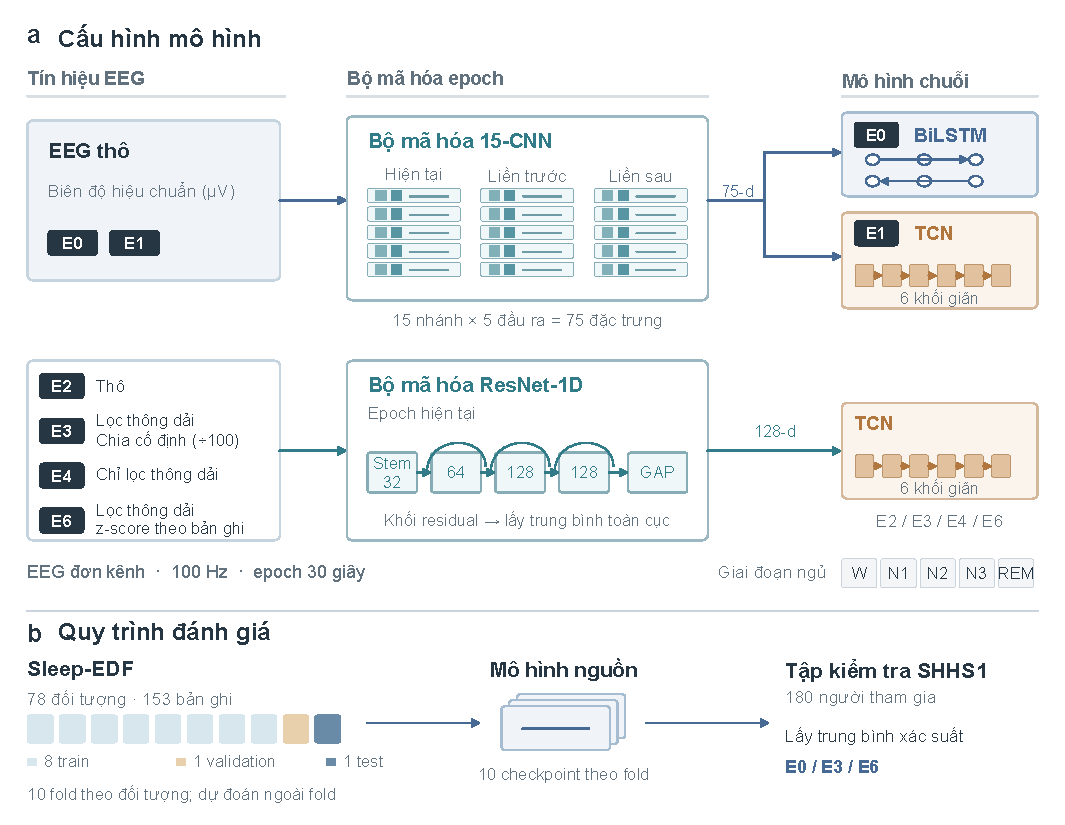
\includegraphics[width=\textwidth]{figures/study_design_vi.pdf}
\caption{\textbf{Các cấu hình mô hình và quy trình đánh giá.} (a) E0 và E1 dùng chung bộ mã hóa 15-CNN: năm nhánh cho mỗi epoch hiện tại, liền trước và liền sau tạo thành 75 đặc trưng cho BiLSTM hoặc TCN. E2, E3, E4 và E6 dùng bộ mã hóa ResNet-1D cho epoch hiện tại, được huấn luyện riêng theo từng cấu hình, cùng TCN. Các số trong ResNet biểu thị số kênh đầu ra; GAP là phép lấy trung bình toàn cục. Cả hai TCN đều có sáu khối tích chập giãn không nhân quả. E3 và E6 còn cắt biên độ tại $\pm800\,\mu$V sau lọc thông dải; E3 chia cho 100, còn E6 dùng thống kê z-score của toàn bản ghi. (b) Sleep-EDF dùng mười fold theo đối tượng, chung cho các cấu hình; mỗi lượt gồm tám fold huấn luyện, một fold xác thực và một fold kiểm tra. Đánh giá chính trên SHHS1 so sánh E0, E3 và E6 trên 180 người tham gia, lấy trung bình xác suất từng lớp từ mười checkpoint nguồn trước khi chọn lớp dự đoán, không huấn luyện mô hình trên miền đích. E6 dùng thống kê bản ghi đích không nhãn. E5 chỉ kiểm tra tính đồng nhất của đầu vào, không phải một cấu hình đánh giá hiệu năng bổ sung. Thiết lập huấn luyện và các phân tích bổ sung được mô tả trong phần Phương pháp và tài liệu bổ sung. Sơ đồ được vẽ bằng Matplotlib với sự hỗ trợ của OpenAI Codex; các ký hiệu biểu diễn cấu trúc mô hình và vai trò của fold, không phải tín hiệu đo hay kích thước phân hoạch.}
\label{fig:pipeline}
\end{figure}

Mọi điều kiện đều tác động lên tín hiệu liên tục đã hiệu chuẩn theo microvolt trước khi chia epoch. Bốn điều kiện tín hiệu được đưa vào phân tích hiệu năng; một điều kiện chỉ phục vụ kiểm tra (E5) ghi nhận thí nghiệm đối chiếu bước giới hạn biên độ đã được dự kiến:

\begin{itemize}
\item \textbf{Tín hiệu thô} (E0--E2): không lọc, không giới hạn biên độ, không đổi thang; giữ đơn vị $\mu$V gốc.
\item \textbf{Chỉ lọc thông dải} (E4): bộ lọc Butterworth thông dải không lệch pha, bậc 4, 0.5--30\,Hz, triển khai bằng các tầng bậc hai với phép lọc tiến--lùi.
\item \textbf{Lọc thông dải và giới hạn biên độ} (E5; chỉ kiểm tra): tín hiệu E4 tiếp tục được chặn cứng ở $\pm800\,\mu$V. Trên toàn bộ 153 bản ghi Sleep-EDF, E5 và E4 giống nhau từng bit, và tỷ lệ mẫu bị giới hạn đo được bằng không. Fold 0 được giữ làm hiện vật kiểm tra; các fold còn lại và mọi kiểm định hiệu năng bị hủy trước khi xem điểm số vì E5 không tạo ra một điều kiện đầu vào độc lập.
\item \textbf{Xử lý biên độ bằng hệ số cố định} (E3): cùng phép lọc thông dải, sau đó chặn cứng ở $\pm800\,\mu$V và chia cho hằng số 100. Ngưỡng giới hạn là hằng số tuyệt đối giống nhau cho mọi bản ghi, nên không ước lượng thống kê ở cấp bản ghi hay quần thể và không tạo rò rỉ giữa các đối tượng; quan hệ biên độ tương đối giữa các bản ghi được giữ lại.
\item \textbf{Chuẩn hóa $z$-score theo bản ghi} (E6): cùng phép lọc và giới hạn, sau đó trừ trung bình và chia cho độ lệch chuẩn tính trên toàn bộ bản ghi đã lọc và giới hạn. Cách này không dùng nhãn đích nhưng dùng toàn bộ mẫu tín hiệu của bản ghi đích, loại bỏ khác biệt biên độ tuyệt đối giữa các bản ghi và có tính transductive ở cấp bản ghi, thay vì thuần túy quy nạp.
\end{itemize}

Không áp dụng bộ lọc notch: 50\,Hz nằm ngoài dải thông 0.5--30\,Hz và tại tần số Nyquist của tín hiệu 100\,Hz. Vì vậy, đối chiếu E3\,--\,E6 đánh giá một lựa chọn tiền xử lý thực tế: giữ quan hệ biên độ đã hiệu chuẩn giữa các bản ghi hay chuẩn hóa từng bản ghi. Do bước giới hạn không bao giờ được kích hoạt trong kiểm tra E5 trên Sleep-EDF, E3 và E4 trên Sleep-EDF chỉ khác nhau ở phép chia cố định cho 100; kiểm tra tương ứng trên SHHS cũng không ghi nhận mẫu nào bị giới hạn. Vì vậy, so sánh E3--E4 kiểm tra huấn luyện và đánh giá ở hai thang đầu vào trên những dữ liệu này, không phải tác động của một bước giới hạn biên độ thực sự có hiệu lực.

\subsection{Cấu hình mô hình}

\begin{table}[htbp]
\centering
\caption{Mã cấu hình thực nghiệm. Mã biểu thị tổ hợp tín hiệu và mô hình, không phải thứ hạng hiệu năng hay thứ tự phiên bản mô hình.}
\label{tab:configs}
\small
\begin{tabularx}{\textwidth}{lYYY}
\toprule
\textbf{ID} & \textbf{Điều kiện tín hiệu} & \textbf{Bộ mã hóa epoch} & \textbf{Mô hình chuỗi và vai trò} \\
\midrule
E0 & Thô & CNN 15 nhánh & BiLSTM; đối chứng nội bộ \\
E1 & Thô & CNN 15 nhánh & TCN; thay mô hình chuỗi và thiết lập huấn luyện \\
E2 & Thô & ResNet-1D & TCN; thay bộ mã hóa/ngữ cảnh và huấn luyện bộ mã hóa \\
E3 & Lọc dải + giới hạn + đổi thang cố định & ResNet-1D & TCN; cấu hình đổi thang cố định \\
E4 & Chỉ lọc thông dải & ResNet-1D & TCN; cấu hình lọc thông dải \\
E5 & Lọc dải + giới hạn & ResNet-1D & TCN; chỉ kiểm tra, đầu vào giống E4 \\
E6 & Lọc dải + giới hạn + $z$-score & ResNet-1D & TCN; cách đổi thang thay thế \\
\bottomrule
\end{tabularx}
\end{table}

Sáu cấu hình hoạt động (E0--E4 và E6) tham gia phân tích hiệu năng; E5 ghi nhận đối chiếu riêng bước giới hạn biên độ đã bị hủy. Bộ mã hóa đối chứng ghép đầu ra softmax năm lớp từ 15 nhánh CNN bao phủ epoch hiện tại, trước và sau (C/P/N), tạo 75 đặc trưng cho mỗi epoch trung tâm. Ngữ cảnh luôn nằm trong từng bản ghi; tại biên, epoch đầu hoặc cuối được lặp lại. ResNet-1D tạo 128 đặc trưng chỉ từ epoch hiện tại. TCN không nhân quả gồm sáu khối có trường tiếp nhận 253 epoch; BiLSTM đối chứng có 128 đơn vị ẩn theo mỗi chiều. Cả hai mô hình chuỗi xử lý phần bản ghi được giữ lại với phần đệm có mặt nạ. Đây là các mô hình ngoại tuyến: BiLSTM và TCN sử dụng ngữ cảnh tương lai, còn lọc không lệch pha và chuẩn hóa E6 sử dụng mẫu tín hiệu tương lai. Benchmark truyền xuôi không đo độ trễ ra quyết định trực tuyến. Kích thước các lớp và toàn bộ siêu tham số được trình bày trong phần Phương pháp bổ sung S1.

\subsection{Huấn luyện hai giai đoạn và đánh giá chéo theo đối tượng}

78 đối tượng được chia thành 10 fold không trùng đối tượng. Trong mỗi lượt đánh giá, một fold là tập kiểm tra (test), fold kế tiếp (theo modulo 10) là tập xác thực (validation), và các fold còn lại là tập huấn luyện. Cả hai đêm của cùng một đối tượng luôn có cùng vai trò. Mọi cấu hình dùng cùng phép chia; fold test không bao giờ tham gia lựa chọn mô hình. Giao diện huấn luyện chỉ nhận bộ nạp dữ liệu huấn luyện và xác thực; huấn luyện bộ mã hóa và lưu đặc trưng cũng tuân theo cùng cách gán đối tượng vào fold.

Huấn luyện gồm hai giai đoạn. Bộ mã hóa epoch dùng trọng số lớp tính từ các đối tượng huấn luyện và được chọn trên dữ liệu xác thực: tối thiểu hóa mất mát xác thực có trọng số với từng CNN đối chứng, và tối đa hóa \mf\ xác thực với ResNet. Checkpoint được chọn được kiểm tra mã băm rồi dùng để lưu đặc trưng mà không tính gradient. Mô hình chuỗi được huấn luyện trên bộ đặc trưng đã đóng băng bằng cross-entropy có mặt nạ và được chọn theo \mf\ xác thực. E1 dùng lại checkpoint bộ mã hóa E0 nhưng thay thiết lập bộ tối ưu của mô hình chuỗi: lần lượt với E0 và E1, tốc độ học là 0.01 và 0.0005, kích thước batch là 4 và 8 bản ghi, số epoch huấn luyện tối đa là 1{,}000 và 300, còn patience là 10 và 30. E2 còn thay cách tối ưu và lựa chọn bộ mã hóa cùng với việc thay gói đặc trưng/ngữ cảnh. Phần Phương pháp bổ sung S1 trình bày đầy đủ các thiết lập. Vì vậy, các so sánh giữ nguyên phép chia đối tượng và cách đánh giá, chứ không giữ nguyên mọi lựa chọn huấn luyện.

\subsection{Phân tích thống kê và giao thức đánh giá}

Cả sáu cấu hình hoàn tất việc lựa chọn dựa trên tập xác thực trước khi đánh giá dự đoán test của đợt chính với seed 42. Trên Sleep-EDF, \mf\ gộp là chỉ số mô tả chủ đạo, nhưng đơn vị suy luận thống kê là đối tượng. Bootstrap bắt cặp theo cụm đối tượng với 10{,}000 lần lấy mẫu lại ước lượng khoảng tin cậy phân vị cho chênh lệch \mf\ gộp~\cite{efron1994bootstrap}; kiểm định hạng có dấu Wilcoxon hai phía~\cite{wilcoxon1945} đánh giá phân bố chênh lệch theo từng đối tượng. Hiệu chỉnh Holm~\cite{holm1979} được áp dụng cho bốn so sánh xác định trước: E1\,--\,E0, E2\,--\,E1, E3\,--\,E2 và E3\,--\,E6. \mf\ gộp được tính từ tổng các ma trận nhầm lẫn của đối tượng; \mf\ trung bình theo đối tượng là trung bình số học các điểm của từng người. Hai đại lượng không thể dùng thay thế nhau, và \mf\ gộp không phải trung bình có trọng số của các giá trị \mf\ riêng lẻ. Khoảng bootstrap mô tả chênh lệch điểm gộp, còn Wilcoxon đánh giá các chênh lệch bắt cặp theo đối tượng qua hạng có dấu. Mọi khoảng bootstrap đều là khoảng tin cậy biên 95\%, không phải các khoảng đồng thời đã hiệu chỉnh cho nhiều so sánh. Phần Phương pháp bổ sung S1 nêu seed bootstrap và cách xử lý chênh lệch bằng không. Các chỉ số dùng cố định năm lớp và gán giá trị bằng không khi mẫu số theo lớp bằng không. Trong phân tích Sleep-EDF, E3\,--\,E0 luôn được ghi rõ là hậu nghiệm.

Chúng tôi cũng báo cáo số đối tượng thắng/hòa/thua, độ trội về dấu $(W-L)/(W+L)$ và kiểm định dấu chính xác chưa hiệu chỉnh như các kiểm tra độ vững mang tính mô tả; chúng không thuộc họ kiểm định suy luận xác định trước. Ở đây, W/T/L lần lượt là số đối tượng có điểm tăng/không đổi/giảm.

Đợt thực nghiệm seed 123 đã hoàn tất lặp lại phép đánh giá với seed huấn luyện cố định thứ hai trên cùng phép chia. Hai seed được phân tích riêng; không bao giờ gộp các giá trị $p$, và hai seed cố định không mô tả được phân bố theo các khởi tạo. Chúng tôi báo cáo lần lặp này như bằng chứng về độ nhạy, không phải một đợt kiểm chứng xác nhận bổ sung. Cấu hình lưu trữ liệt kê các seed 42, 123 và 2025; chỉ hai đợt đã hoàn thành với seed 42 và 123 đóng góp kết quả ở đây.

Với SHHS, mỗi cấu hình sử dụng cả mười checkpoint từ các fold ngoài của Sleep-EDF. Xác suất softmax được lấy trung bình giữa các fold bằng float64 trước khi chọn argmax cuối cùng cho từng epoch. Tiêu chí chính được xác định trước là \mf\ trung bình theo đối tượng, với E3\,--\,E0 và E3\,--\,E6 là hai so sánh chính, áp dụng cùng cách bootstrap theo cụm đối tượng và Wilcoxon--Holm; trong trường hợp này, khoảng bootstrap dành cho chênh lệch trung bình theo đối tượng. Phân tích E1/E2 là bằng chứng thứ cấp trên mẫu đã được mở kết quả, và E3\,--\,E2 được ghi rõ là hậu nghiệm. Phần mở rộng E4 với seed 123 có họ hiệu chỉnh Holm riêng gồm bốn so sánh, được báo cáo trong tài liệu bổ sung. Phân tích vùng ranh giới nhãn tham chiếu và vùng ổn định là các phân tích chẩn đoán ngoại tuyến hậu nghiệm; mặt nạ, quy tắc loại trừ và số lượng epoch tương ứng được xác định chính xác trong phần Phương pháp bổ sung S1.

\subsection{Các thí nghiệm can thiệp bổ sung}

Sau khi phân tích sai số trên SHHS1, chúng tôi đánh giá hiệu chuẩn nhiệt độ kết hợp hiệu chỉnh tiên nghiệm bằng EM, huấn luyện TCN với trọng số lớp và một so sánh ADAST theo giao thức chung~\cite{eldele2023adast}. Các thí nghiệm tiếp theo này dùng lại cùng 180 người tham gia SHHS1. Hiệu chuẩn sử dụng đủ mười fold E3 seed 123: mỗi nhiệt độ được khớp trên tập xác thực nguồn, mỗi tiên nghiệm EM được ước lượng từ năm người adaptation cố định không nhãn, tách biệt với test. Trọng số lớp sử dụng mười cặp seed 123: mỗi fold giữ nguyên bộ mã hóa E3 lịch sử đã đóng băng và huấn luyện lại đối chứng không trọng số tương ứng. Hai nhánh đều lấy trung bình xác suất của đủ mười fold. Fold 0--5 được huấn luyện trên CPU, fold 6--9 trên CUDA; thời gian này không được đưa vào benchmark vận hành lịch sử. Kết quả fold 0 ban đầu được giữ riêng. ADAST sử dụng mười cặp mới được huấn luyện trên CUDA, seed 123, với đối chứng source-only hai bộ phân loại tương ứng trong mỗi fold. Mỗi nhánh có 1.140 update mỗi fold và lấy trung bình xác suất đủ mười fold; kết quả outer test nguồn là dự đoán ngoài fold, không phải tổ hợp. Pilot ADAST một fold trên CPU trước đây được giữ riêng, không gộp vào lượt CUDA. Mọi nhánh suy luận toàn bản ghi đích trước khi áp cùng mặt nạ chấm điểm lịch sử; vì vậy hiệu chuẩn dùng đối chứng E3 toàn bản ghi được chạy lại. Mô hình được chọn bằng validation nguồn; thích nghi dùng dữ liệu đích không nhãn; nhãn test đích được dùng để chấm điểm. Phần Phương pháp bổ sung S2 nêu cách khớp, chọn mô hình và ngân sách thích nghi. Khoảng bootstrap bắt cặp theo người của các thí nghiệm này được báo cáo riêng với kiểm định chính.

Các thí nghiệm phát triển tiếp theo trên fold nguồn 0 (seed 123) so sánh ngân sách 1.140 với 36.870 update mỗi mô hình, sau đó chạy một đối chứng ADAST toàn nguồn mới và ba can thiệp riêng vào thành phần loss. Tất cả mô hình chạy 30 epoch trên T4 CUDA. Checkpoint được chọn theo \mf\ lớn nhất trên validation nguồn qua source attention, giữ epoch đầu tiên khi bằng điểm; checkpoint epoch 30 được báo riêng. Năm người adaptation không nhãn được dùng lại, không truy cập outer test nguồn hoặc SHHS test. Cả hai đường attention đều được đánh giá trên cùng validation nguồn. Các so sánh phát triển này tách biệt với đánh giá chuyển quần thể mười fold (Bảng bổ sung~\ref{SM-tab:sup_adast_budget_development} và~\ref{SM-tab:sup_adast_loss_development}).

Một lượt kiểm tra ba nhánh tiếp theo dùng fold nguồn 1 với cùng seed, so sánh ba mô hình mới: source-only, ADAST đối chứng và ADAST giữ hệ số loss nguồn. Mỗi mô hình có 35.820 update trong 30 epoch, học đủ 152.825 đoạn train nguồn ở mỗi lượt. Vai trò dữ liệu chọn checkpoint và thích nghi được giữ nguyên; validation nguồn có 23.881 đoạn. Cả hai đường attention được đánh giá tại checkpoint được chọn và checkpoint epoch 30 (Bảng bổ sung~\ref{SM-tab:sup_adast_confirmation} và~\ref{SM-tab:sup_adast_confirmation_attention}).

Để khảo sát độ nhạy khi chuyển quần thể theo ngân sách học, chúng tôi hoàn thiện mười cặp toàn nguồn ở seed 123: 16 mô hình mới cho fold nguồn 2--9 và bốn mô hình tương thích dùng lại từ fold 0--1, không lấy các nhánh can thiệp loss. Mỗi mô hình học 30 lượt đầy đủ tập train nguồn, tương ứng 35.670--37.620 update tùy fold; hai nhánh trong mỗi cặp có cùng khởi tạo và thứ tự nguồn. ADAST dùng lại đúng năm người adaptation không nhãn. Ngân sách toàn nguồn đồng thời tăng số lần xem target và thay đổi thời điểm scheduler theo đơn vị update; đây là so sánh ngân sách học, không phải can thiệp cô lập độ phủ nguồn. So sánh chính dùng checkpoint epoch 30 cho cả hai nhánh ở cả hai ngân sách. Hai logits đầu ra được lấy cực đại rồi softmax trong mỗi fold, sau đó lấy trung bình xác suất đủ mười fold; SHHS dùng source attention cho source-only và target attention cho ADAST. Outer test Sleep-EDF dùng đúng fold tương ứng và source attention cho cả hai nhánh. Chúng tôi tính ADAST trừ source-only ở mỗi ngân sách và chênh lệch giữa hai hiệu ứng, dùng chung 10.000 lượt bootstrap theo người ở cả bốn hệ thống. Các khoảng này điều kiện trên mô hình đã học, không bao gồm biến thiên huấn luyện (Bảng~\ref{tab:adast-budget-main}; Bảng bổ sung~\ref{SM-tab:sup_adast_fullsource_classes}).

Trong đánh giá phụ toàn nguồn, mỗi mô hình dùng checkpoint có \mf\ lớn nhất trên validation nguồn qua source attention, giữ epoch đầu tiên khi bằng điểm. Đường attention, cách kết hợp và chấm điểm không đổi; nhãn SHHS không tham gia lựa chọn.

\subsection{Đánh giá vận hành}

Thời gian suy luận được đo trên cùng phần cứng (Tesla V100) cho mọi cấu hình, không bao gồm vào/ra dữ liệu, tiền xử lý và huấn luyện. Mỗi phép đo dùng một batch gồm một chuỗi tổng hợp 100 epoch, 20 lượt làm nóng và ba vòng, mỗi vòng 100 lượt truyền xuôi có đo thời gian. Thứ tự cấu hình được xáo trộn trong từng vòng; chúng tôi báo cáo trung vị của toàn bộ 300 lượt. Benchmark đo quy trình truyền xuôi đầy đủ đã triển khai với một kích thước tensor cố định, không đo thời gian suy luận thực tế cho cả đêm hay độ phức tạp thuật toán.

Hình biểu diễn tốc độ và hiệu năng kết hợp điểm tổng hợp ở seed 42 với hệ số tăng tốc truyền xuôi đo được; hai ô hình phân biệt điểm gộp trên Sleep-EDF với điểm trung bình theo đối tượng trên SHHS1.

%==============================================================================
\section{Kết quả}

\subsection{Hiệu năng ngoài fold trên Sleep-EDF}

\begin{table}[htbp]
\centering
\caption{Hiệu năng kiểm tra ngoài fold trên Sleep-EDF (seed 42, gộp toàn bộ các fold).}
\label{tab:sleepedf-performance}
\small
\begin{tabular}{lrrrr}
\toprule
\textbf{Cấu hình} & \textbf{\mf} & \textbf{Độ chính xác} & \textbf{$\kappa$} & \textbf{F1 (N1)} \\
\midrule
E0 & 0.7754 & 0.8262 & 0.7614 & 0.5009 \\
E1 & 0.7802 & 0.8315 & 0.7683 & 0.5115 \\
E2 & 0.7835 & 0.8341 & 0.7716 & 0.5180 \\
E3 & \textbf{0.7904} & \textbf{0.8363} & \textbf{0.7754} & \textbf{0.5276} \\
E4 & 0.7891 & 0.8360 & 0.7746 & 0.5270 \\
E6 & 0.7691 & 0.8230 & 0.7573 & 0.5124 \\
\bottomrule
\end{tabular}
\end{table}

E3 dẫn đầu đợt thực nghiệm chính seed 42 ở cả bốn chỉ số (Bảng~\ref{tab:sleepedf-performance}); kết quả bắt cặp được báo cáo trong Bảng~\ref{tab:paired-sleepedf}.

\begin{table}[htbp]
\centering
\caption{Các so sánh bắt cặp xác định trước trên \mf\ của Sleep-EDF ($n = 78$ đối tượng). Hiệu chỉnh Holm áp dụng cho bốn dòng xác định trước; thống kê kiểm định dấu là kiểm tra độ vững bổ sung chưa hiệu chỉnh. E3\,--\,E0 là hậu nghiệm và không thuộc họ Holm. W/T/L: thắng/hòa/thua; $\dsign$: độ trội về dấu.}
\label{tab:paired-sleepedf}
\small
\resizebox{\textwidth}{!}{%
\begin{tabular}{lrrrrrr}
\toprule
\textbf{So sánh} & $\boldsymbol{\Delta}$\textbf{\mf} & \textbf{\ci} & $\boldsymbol{p_{\mathrm{Holm}}}$ & \textbf{W/T/L} & $\boldsymbol{\dsign}$ & $\boldsymbol{p_{\mathrm{sign}}}$ \\
\midrule
E1\,--\,E0 & 0.004811 & $[-0.000915, 0.010193]$ & 0.1022 & 51/0/27 & $+0.308$ & 0.0088 \\
E2\,--\,E1 & 0.003251 & $[-0.002370, 0.008808]$ & 0.1036 & 44/0/34 & $+0.128$ & 0.3082 \\
E3\,--\,E2 & 0.006962 & $[0.000305, 0.014520]$  & 0.8989 & 37/0/41 & $-0.051$ & 0.7343 \\
E3\,--\,E6 & \textbf{0.021319} & $\boldsymbol{[0.012179, 0.030698]}$ & \textbf{0.0012} & 49/0/29 & $\boldsymbol{+0.256}$ & \textbf{0.0308} \\
\midrule
\textit{E3\,--\,E0 (hậu nghiệm)} & 0.015024 & $[0.005746, 0.025871]$ & --- & 49/0/29 & $+0.256$ & 0.0308 \\
\bottomrule
\end{tabular}}
\end{table}

Trong các đối chiếu xác định trước, chỉ E3\,--\,E6 đồng thời có khoảng bootstrap của chỉ số gộp hoàn toàn dương ($[0.012179, 0.030698]$) và kết quả Wilcoxon cấp đối tượng có ý nghĩa sau hiệu chỉnh Holm ($p=0.0012$). Khoảng của E1\,--\,E0 và E2\,--\,E1 đều chứa không. E3\,--\,E2 có khoảng gộp dương ($[0.000305, 0.014520]$) nhưng Wilcoxon sau Holm không có ý nghĩa ($p=0.8989$), chỉ cải thiện ở 37 trong 78 đối tượng ($\dsign=-0.051$; $p_{\mathrm{sign}}=0.734$). Kết quả này ủng hộ một cải thiện nhỏ ở điểm gộp, thay vì lợi thế nhất quán ở cấp đối tượng. Đối chiếu hậu nghiệm E3\,--\,E0 tăng $0.0150$ \mf\ so với E0, với khoảng $[0.005746, 0.025871]$; chênh lệch này đại diện cho thay đổi kết hợp của kiến trúc, tiền xử lý và cấu hình huấn luyện.

\subsection{Kiểm tra theo lớp và độ nhạy theo seed}

Các chỉ số chi tiết theo lớp, ma trận nhầm lẫn Sleep-EDF và cả hai bảng kiểm tra độ nhạy theo seed được trình bày ở các Bảng bổ sung~\ref{SM-tab:sup_edf_perclass}--\ref{SM-tab:sup_edf_seed_contrasts}. Trong miền, N1 là lớp khó nhất của E3, còn chênh lệch F1 E3--E6 lớn nhất nằm ở N3 ($+0.0628$). Cả bốn chênh lệch xác định trước vẫn dương với seed 123, nhưng chỉ E3\,--\,E6 có khoảng bootstrap hoàn toàn dương ở cả hai lần chạy; kết quả sau Holm chỉ có ý nghĩa ở seed 42, và độ lớn giảm từ 0.0213 xuống 0.0102. Vì vậy, chiều chênh lệch ổn định qua hai seed cố định, còn mức độ bằng chứng suy luận thì không.

\FloatBarrier
\subsection{Độ phức tạp, độ trễ và chi phí huấn luyện}

\begin{table}[htbp]
\centering
\caption{Benchmark truyền xuôi toàn quy trình trên Tesla V100 (fold 0, seed 42; batch 1, độ dài chuỗi 100). Thông lượng có đơn vị epoch\,s$^{-1}$; bộ nhớ cấp phát cực đại có đơn vị MiB; không gồm vào/ra dữ liệu và tiền xử lý.}
\label{tab:complexity}
\small
\begin{tabular}{lrrrrr}
\toprule
\textbf{ID} & \textbf{Số tham số} & \textbf{Trung vị (ms)} & \textbf{Thông lượng} & \textbf{Bộ nhớ đỉnh} & \textbf{Tăng tốc} \\
\midrule
E0 & 248{,}630 & 13.4315 & 7{,}445 & 58.81 & $1.00\times$ \\
E1 & 640{,}950 & 12.5111 & 7{,}993 & 60.31 & $1.07\times$ \\
E2 & 1{,}085{,}578 & 3.5750 & 27{,}972 & 75.54 & $3.76\times$ \\
E3 & 1{,}085{,}578 & 3.5687 & 28{,}021 & 75.54 & $3.76\times$ \\
E6 & 1{,}085{,}578 & 3.5756 & 27{,}967 & 75.54 & $3.76\times$ \\
\bottomrule
\end{tabular}
\end{table}

Như Bảng~\ref{tab:complexity} cho thấy, họ ResNet-1D--TCN đạt hệ số tăng tốc đo được $3.76\times$ so với đối chứng CNN--BiLSTM dù có số tham số gấp $4.37\times$. Bộ nhớ cấp phát cực đại là 75.54 MiB so với 58.81 MiB ở đối chứng, tức tăng tuyệt đối 16.73 MiB trong benchmark này. Hình~\ref{fig:speedup_tradeoff} tóm tắt đánh đổi tốc độ--hiệu năng đo được cho các cấu hình chính E0, E3 và E6 ở seed 42. Trên mẫu SHHS1, E3 kết hợp tốc độ truyền xuôi nhanh hơn với kết quả tổng hợp cao hơn E0 và E6. Vì vậy, cách triển khai này nhanh hơn nhưng không nhỏ hơn. Trong benchmark truyền xuôi, E1 dùng lại bộ mã hóa của E0 và thay mô hình chuỗi, đạt hệ số tăng tốc $1.07\times$. Mức tăng tốc lớn hơn của E2 so với E0 đi cùng việc thay 15 nhánh CNN thực thi độc lập bằng một bộ mã hóa ResNet-1D trong quy trình đã triển khai.

\begin{figure}[htbp]
\centering
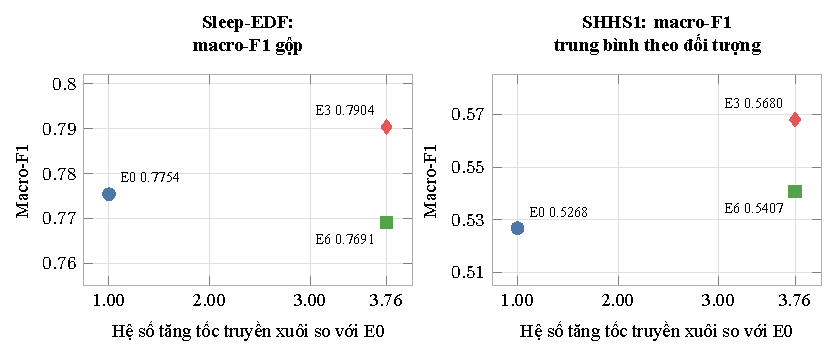
\includegraphics[width=0.94\textwidth]{figures/speedup_vi.pdf}
\caption{\textbf{Hệ số tăng tốc truyền xuôi đo được và \mf\ tổng hợp của các cấu hình chính seed 42.} Chỉ biểu diễn E0, E3 và E6. Ô bên trái báo cáo \mf\ gộp trên Sleep-EDF; ô bên phải báo cáo \mf\ trung bình theo đối tượng trên mẫu SHHS1. Hệ số tăng tốc được tính so với E0 trong benchmark truyền xuôi cố định. Biểu đồ được tạo từ kết quả tổng hợp đã lưu bằng mã PGFPlots có thể chỉnh sửa; OpenAI Codex hỗ trợ viết mã vẽ.}
\label{fig:speedup_tradeoff}
\end{figure}

\FloatBarrier

Trong đợt thực nghiệm seed 123 chạy tuần tự, toàn bộ quá trình huấn luyện và đánh giá xác thực của E2 và E3 được ghi nhận nhanh hơn E0 lần lượt 12.2$\times$ và 10.2$\times$. E1 dùng lại checkpoint bộ mã hóa E0 nên không có so sánh thời gian từ đầu đến cuối. Thời gian đầy đủ theo các thiết lập huấn luyện và dừng sớm đã xác định được báo cáo trong Bảng bổ sung~\ref{SM-tab:sup_seed123_runtime}.

\FloatBarrier

Các phân tích mô tả bổ sung về biểu diễn và nhóm ngữ cảnh được báo cáo trong Hình bổ sung~\ref{SM-fig:sup_representation_context} và Bảng~\ref{SM-tab:sup_context}; chúng cung cấp bằng chứng bổ trợ về hình học đặc trưng và ngữ cảnh thời gian. Trong thí nghiệm loại bỏ ngữ cảnh của E1 trên Sleep-EDF, thêm các nhóm đặc trưng tường minh của epoch trước và sau (P/N) vào đặc trưng epoch hiện tại không tạo ra cải thiện hiệu năng vùng ranh giới có thể phát hiện được ($\Delta\mf=0.0010$, \ci\ $[-0.0046,0.0066]$, Holm $p=1.000$; 36/78 đối tượng cải thiện). Kết quả này chỉ áp dụng trong điều kiện mã hóa E1 và thiết lập TCN đã xác định.

\subsection{Đánh giá chuyển quần thể trên SHHS1}
\label{sec:shhs}

\begin{table}[htbp]
\centering
\caption{Hiệu năng chuyển quần thể trên 180 người tham gia SHHS1 (seed 42). Mọi trọng số mô hình được huấn luyện trên Sleep-EDF. E6 còn dùng thống kê của toàn bản ghi đích không nhãn. Các khoảng là khoảng bootstrap theo cụm đối tượng cho \mf\ trung bình theo đối tượng.}
\label{tab:shhs-performance}
\small
\begin{tabular}{lrrrr}
\toprule
\textbf{ID} & \textbf{\mf\ TB theo đối tượng (\ci)} & \textbf{\mf\ gộp} & \textbf{Độ chính xác} & \textbf{$\kappa$} \\
\midrule
E0 & 0.5268 \ $[0.5101, 0.5431]$ & 0.5761 & 0.6648 & 0.5339 \\
E3 & \textbf{0.5680} \ $\boldsymbol{[0.5503, 0.5850]}$ & \textbf{0.6099} & \textbf{0.7016} & \textbf{0.5801} \\
E6 & 0.5407 \ $[0.5227, 0.5584]$ & 0.5732 & 0.6742 & 0.5408 \\
\bottomrule
\end{tabular}
\end{table}

Đợt seed 123 giữ nguyên chiều chênh lệch và ý nghĩa sau Holm của cả hai đối chiếu SHHS, trong khi so sánh E3\,--\,E6 trong miền không còn đạt ngưỡng Holm. Kết quả kiểm tra độ nhạy này sử dụng cùng mẫu SHHS; họ kiểm định mở rộng gồm bốn so sánh được báo cáo riêng trong tài liệu bổ sung.

\begin{table}[htbp]
\centering
\caption{Các so sánh bắt cặp chính trên \mf\ trung bình theo đối tượng của SHHS1 ($n = 180$).}
\label{tab:shhs-paired}
\small
\resizebox{\textwidth}{!}{%
\begin{tabular}{llrrrrr}
\toprule
\textbf{So sánh} & \textbf{Vai trò} & $\boldsymbol{\Delta}$ & \textbf{\ci} & $\boldsymbol{p_{\mathrm{Holm}}}$ & \textbf{W/T/L} & $\boldsymbol{\dsign}$ \\
\midrule
E3\,--\,E0 & chính & 0.0412 & $[0.0314, 0.0512]$ & $2.65\times10^{-13}$ & 138/0/42 & $+0.533$ \\
E3\,--\,E6 & chính & 0.0274 & $[0.0182, 0.0370]$ & $1.87\times10^{-8}$ & 125/0/55 & $+0.389$ \\
\bottomrule
\end{tabular}}
\end{table}

Cả hai so sánh chính đều ủng hộ E3 (Bảng~\ref{tab:shhs-paired}), với cải thiện lần lượt ở 138 và 125 trong 180 đối tượng. Độ trội về dấu là $+0.533$ và $+0.389$; kiểm định dấu chính xác chưa hiệu chỉnh cho $p = 3.8\times10^{-13}$ và $1.9\times10^{-7}$. Các chỉ số hỗ trợ cùng thay đổi theo hướng thuận lợi: so với E0, E3 tăng $0.0338$ \mf\ gộp, $0.0368$ độ chính xác và $0.0461$ $\kappa$. Trong phạm vi $\pm1$ epoch quanh chuyển đổi nhãn tham chiếu, \mf\ gộp vùng ranh giới của E3 cao hơn E0 $0.0366$ và cao hơn E6 $0.0183$.

Phân tích cấu hình thứ cấp cho thấy một bức tranh khác. E1\,--\,E0 vẫn dương nhưng nhỏ ($+0.0065$ \mf\ trung bình theo đối tượng). E2\,--\,E1 là \emph{âm} ngoài miền ($-0.0128$, khoảng tin cậy hoàn toàn dưới không), nên việc thay đồng thời gói C/P/N 75 chiều của E1 bằng biểu diễn ResNet-1D 128 chiều từ epoch hiện tại không tổng quát hóa tốt hơn trên tín hiệu SHHS chưa xử lý. Vì toàn bộ gói đặc trưng/ngữ cảnh thay đổi, không thể quy sự đảo chiều này riêng cho bộ mã hóa. Đối chiếu hậu nghiệm E3\,--\,E2 là chênh lệch lớn nhất trong các khác biệt cấu hình được báo cáo ở phần mở rộng SHHS1 này ($+0.0475$, \ci\ $[0.0372,0.0579]$, $\dsign = +0.633$, 147/180 đối tượng cải thiện). E3 và E2 dùng cùng mô hình và thiết lập huấn luyện đã xác định nhưng khác tiền xử lý. Chênh lệch quan sát được này lớn hơn cả đối chiếu mô hình chuỗi/thiết lập huấn luyện lẫn đối chiếu bộ mã hóa/ngữ cảnh trên mẫu này.

Phần mở rộng seed 123 đánh giá E4 (chỉ lọc thông dải) cung cấp một đối chiếu thứ cấp cụ thể hơn. E4 đạt \mf\ trung bình theo đối tượng $0.5732$, \mf\ gộp $0.6147$, độ chính xác $0.7064$, $\kappa = 0.5869$ và F1 N1 $0.3492$, cao hơn E2 cùng seed $0.0323$ và cao hơn E3 ($0.5634$) $0.0098$ (\ci\ bắt cặp $[0.0073,0.0125]$; Holm $p=1.89\times10^{-10}$). Kiểm tra tiền xử lý riêng cho SHHS không ghi nhận mẫu nào bị giới hạn biên độ trên 200 bản ghi đã xử lý thuộc các nhóm adaptation, validation và test. Vì vậy, E4 và E3 trên các đầu vào này chỉ khác ở phép chia cố định cho 100; mỗi cấu hình được huấn luyện riêng trên đầu vào nguồn tương ứng. Trong phần mở rộng này, tiền xử lý chỉ lọc thông dải tốt hơn cả cấu hình tín hiệu thô lẫn cấu hình đổi thang cố định khi dùng cùng seed. Các so sánh vẫn là thứ cấp vì được thực hiện sau khi mẫu SHHS đã được mở kết quả. E4 cũng nhỉnh hơn E3 trên Sleep-EDF ở seed 123 (\mf\ gộp $0.7887$ so với $0.7883$), nên cặp này không cho thấy sự đảo thứ hạng riêng trên SHHS1.

Đánh giá bổ sung ở seed 42 sử dụng đủ mười checkpoint E4 lịch sử được chọn trên nguồn đạt \mf\ trung bình theo đối tượng $0.5811$, so với $0.5680$ của E3 (chênh lệch $0.0131$, \ci\ bắt cặp $[0.0111,0.0153]$). Như vậy, cả hai đối chiếu cùng seed đều nghiêng về E4 trên cùng quần thể SHHS (Bảng bổ sung~\ref{SM-tab:sup_e4_two_seeds}); hai seed không phải hai quần thể độc lập. Dự đoán E3 seed 42 được giữ lại sau khi kiểm tra mã băm và tái chạy đối chiếu số học; phân tích chính ban đầu không thay đổi. Đối chiếu E4 seed 42 dùng đúng cửa sổ benchmark cũ và trung bình đủ mười fold, không xếp hạng theo điểm miền đích; khoảng bootstrap được báo cáo riêng, không thêm giá trị $p$ vào họ kiểm định chính.

Trong phần mở rộng seed 123 này, độ thu hồi N3 gộp của E4 là $0.2591$ và F1 N3 là $0.4068$, so với $0.2410$ và $0.3840$ ở E3. Vì vậy, điểm tổng hợp cao hơn của E4 chỉ lọc thông dải vẫn chưa loại bỏ được tình trạng bỏ sót N3. Phần mở rộng seed 42 cho thấy cùng hạn chế: độ thu hồi N3 và F1 N3 của E4 là $0.2728$ và $0.4233$, so với $0.2582$ và $0.4055$ của E3.

\FloatBarrier
\subsection{Sai số giữa các mô hình và phân bố theo thời gian}
\label{sec:gap}

\mf\ gộp của E3 là $0.7904$ trên Sleep-EDF và $0.6099$ trên SHHS1, chênh lệch $0.1805$. Vì Sleep-EDF dùng dự đoán ngoài fold còn SHHS dùng tổ hợp mười mô hình, chênh lệch $0.1805$ được diễn giải theo nghĩa mô tả. Chúng tôi khảo sát theo lớp và dạng nhầm lẫn để xác định những lỗi còn tồn tại dù E3 có lợi thế tổng hợp khi chuyển miền. Trong toàn bộ phân tích này, A$\rightarrow$B chỉ một epoch có nhãn tham chiếu A nhưng được dự đoán thành B; ký hiệu này không chỉ sự chuyển giai đoạn sinh lý theo thời gian.

N3 là lớp suy giảm mạnh nhất: F1 N3 của E3 giảm từ 0.8085 trên Sleep-EDF xuống 0.4055 trên SHHS1, với độ chuẩn xác (precision) 0.9440 nhưng độ thu hồi (recall) chỉ 0.2582. E0 có độ thu hồi gần tương đương (0.2610) và tỷ lệ N3$\rightarrow$N2 tương tự (72.3\% so với 73.1\% ở E3), cho thấy tình trạng bỏ sót N3 khi chuyển quần thể ở cả hai họ mô hình dù E3 có lợi thế tổng hợp khi chuyển miền (Bảng~\ref{tab:cross-model-n3}). N2$\rightarrow$REM là dạng nhầm lẫn lớn thứ hai của E3.

\begin{table}[htbp]
\centering\small
\caption{Bỏ sót N3 ở các cấu hình SHHS1 chính (seed 42). Mọi mô hình dùng chung 22{,}806 epoch có nhãn tham chiếu N3. Cột cuối là tỷ lệ những epoch này được dự đoán thành N2.}
\label{tab:cross-model-n3}
\begin{tabular}{lrrrrr}
\toprule
\textbf{ID} & \textbf{Precision N3} & \textbf{Recall N3} & \textbf{F1 N3} & \textbf{Số N3$\to$N2} & \textbf{Tỷ lệ} \\
\midrule
E0 & 0.9007 & 0.2610 & 0.4048 & 16{,}480 & 72.3\% \\
E3 & 0.9440 & 0.2582 & 0.4055 & 16{,}674 & 73.1\% \\
E6 & 0.9052 & 0.2005 & 0.3283 & 17{,}764 & 77.9\% \\
\bottomrule
\end{tabular}
\end{table}

Phép tính giả định biết nhãn đúng (oracle) chuyển số lượng trong một ô ngoài đường chéo được chọn của ma trận nhầm lẫn SHHS của E3 sang ô đúng trên đường chéo, rồi tính lại \mf. Sửa N3$\rightarrow$N2 làm \mf\ tăng lên 0.7444; sửa N2$\rightarrow$REM làm điểm tăng lên 0.6596. Những thay đổi này tương ứng với 74.5\% và 27.5\% chênh lệch điểm gộp quan sát được. Phép tính sử dụng nhãn đúng; các tác động phi tuyến này không cộng được với nhau và không phải ước lượng hiệu năng có thể đạt được.

Phân tích chẩn đoán vùng ranh giới nhãn tham chiếu bổ sung thông tin theo thời gian. Với E0 và E3, độ thu hồi N3 gần các điểm đổi nhãn lần lượt là 0.6121/0.6326 trên Sleep-EDF nhưng chỉ 0.0633/0.0733 trên SHHS1. Độ thu hồi tại vùng ổn định của SHHS vẫn thấp, ở mức 0.4008/0.3900. Vì vậy, tình trạng bỏ sót N3 không chỉ nằm trong lân cận ranh giới; không thể mô tả đây thuần túy là lỗi tại các điểm đổi nhãn. Định nghĩa vùng và số lượng epoch được trình bày trong tài liệu bổ sung, bao gồm các epoch bị loại khỏi so sánh vùng gần ranh giới với vùng ổn định.

E6 cung cấp kiểm tra độ nhạy không dùng nhãn nhưng có tính transductive. Cấu hình $z$-score theo bản ghi được huấn luyện riêng có độ thu hồi N3 0.2005, so với 0.2582 của E3; độ thu hồi trong lân cận ranh giới là 0.0721 so với 0.0733. Do đó, tình trạng bỏ sót N3 vẫn tồn tại với cấu hình chuẩn hóa đã thử nghiệm. Kết quả chi tiết theo lớp, nhầm lẫn, oracle và chuyển đổi nhãn nằm trong các Bảng bổ sung~\ref{SM-tab:sup_perclass_transfer}--\ref{SM-tab:sup_boundary}.

%==============================================================================
\subsection{Kết quả thí nghiệm bổ sung}

Trong thí nghiệm hiệu chuẩn mười fold, hiệu chuẩn nhiệt độ thay đổi \mf\ trung bình theo đối tượng từ 0.5590 lên 0.5595 (chênh lệch $0.00049$, \ci\ $[0.00002,0.00097]$). Thêm hiệu chỉnh tiên nghiệm EM làm điểm giảm còn 0.4899 (chênh lệch so với chỉ hiệu chuẩn nhiệt độ $-0.0696$, \ci\ $[-0.0793,-0.0600]$). Cả mười lần khớp EM đều hội tụ nhưng đặt tiên nghiệm N3 gần ngưỡng sàn; tổ hợp không còn dự đoán epoch N3 nào (Bảng bổ sung~\ref{SM-tab:sup_calibration_intervention}). So sánh toàn bản ghi này dùng cùng mười mô hình ở cả ba nhánh, tách biệt với điểm lịch sử từ ngữ cảnh đã cắt.

Trong so sánh trọng số lớp bắt cặp đủ mười fold, độ thu hồi N3 tăng từ 0.2345 lên 0.3225 (chênh lệch $0.0880$, \ci\ $[0.0805,0.0954]$), còn F1 N3 tăng từ 0.3759 lên 0.4795. Tuy nhiên, độ thu hồi N2 giảm từ 0.7260 xuống 0.6728 và độ chính xác giảm từ 0.6892 xuống 0.6663. \mf\ trung bình theo đối tượng thay đổi từ 0.5530 xuống 0.5514 (chênh lệch $-0.0016$, \ci\ $[-0.0049,0.0017]$); \mf\ gộp của nhánh không trọng số/có trọng số là 0.5930/0.5928. Như vậy, trọng số lớp tăng độ thu hồi và F1 N3 nhưng giảm độ thu hồi N2 và độ chính xác; khoảng chênh lệch \mf\ trung bình theo đối tượng chứa giá trị không (Bảng bổ sung~\ref{SM-tab:sup_weighted_intervention}). Trong mỗi fold, hai nhánh dùng chung bộ mã hóa đóng băng, khởi tạo và thứ tự minibatch nguồn. Can thiệp này chỉ huấn luyện bộ phân loại chuỗi, không huấn luyện lại toàn bộ bộ mã hóa; pilot một fold được báo cáo riêng ở Bảng bổ sung~\ref{SM-tab:sup_weighted_pilot}.

So sánh ADAST theo giao thức chung đủ mười fold với ngân sách nhỏ tăng độ thu hồi N3 từ 0.3195 lên 0.4269 (chênh lệch $0.1074$, \ci\ $[0.0714,0.1422]$) và F1 N3 từ 0.4752 lên 0.5837. Tuy nhiên, \mf\ trung bình theo đối tượng giảm từ 0.4949 xuống 0.4497 (chênh lệch $-0.0452$, \ci\ $[-0.0558,-0.0347]$); \mf\ gộp giảm từ 0.5539 xuống 0.5072. ADAST không đưa ra dự đoán N1 nào trên SHHS, trong khi độ thu hồi N1 của đối chứng là 0.1974; độ thu hồi REM cũng giảm từ 0.4343 xuống 0.2938. \mf\ gộp ngoài fold trên nguồn giảm từ 0.6665 xuống 0.5276, nên suy giảm không chỉ xuất hiện trên SHHS. Như vậy, nhận diện N3 cải thiện cùng tổn thất đáng kể ở các giai đoạn khác và giảm hiệu năng tổng hợp. So sánh này dùng seed 123, 1.140 update mỗi mô hình và năm người thích nghi không nhãn (Bảng bổ sung~\ref{SM-tab:sup_adast_intervention}). Pilot một fold trên CPU trước đây (\mf\ trung bình theo đối tượng source-only/ADAST 0.4755/0.4214) được giữ riêng ở Bảng bổ sung~\ref{SM-tab:sup_adast_pilot}.

%==============================================================================
Ở ngân sách toàn nguồn, ADAST tăng \mf\ trung bình theo đối tượng trên SHHS1 từ 0.5010 lên 0.5455 (chênh lệch $0.0445$, \ci\ $[0.0352,0.0539]$), đảo chiều hiệu ứng âm ở ngân sách nhỏ. Chênh lệch giữa hai hiệu ứng ADAST trừ đối chứng là $0.0897$ ($[0.0767,0.1023]$), dựa trên cùng lượt lấy mẫu người ở cả bốn hệ thống (Bảng~\ref{tab:adast-budget-main}). \mf\ gộp tăng từ 0.5478 lên 0.5918. Độ thu hồi N3 tăng từ 0.2432 lên 0.6111 và F1 N3 tăng từ 0.3869 lên 0.7221; tỷ lệ N3$\rightarrow$N2 giảm từ 0.7526 xuống 0.3689.

\begin{table}[htbp]
\centering\small
\caption{So sánh ngân sách học trên 180 người SHHS1 (169.012 epoch chấm điểm). Mọi hàng dùng checkpoint epoch 30 và tổ hợp xác suất mười fold. Source-only là đối chứng tương ứng của ADAST, không phải E3. Toàn nguồn là 30 lượt học đầy đủ tập train.}
\label{tab:adast-budget-main}
\begin{tabular}{llrrrr}
\toprule
Ngân sách & Nhánh & \mf\ theo người & \mf\ gộp & Recall N3 & Recall N1 \\
\midrule
1.140 update & Source-only & .4949 & .5539 & .3195 & .1974 \\
1.140 update & ADAST & .4497 & .5072 & .4269 & .0000 \\
Toàn nguồn & Source-only & .5010 & .5478 & .2432 & .1568 \\
Toàn nguồn & ADAST & .5455 & .5918 & .6111 & .1057 \\
\bottomrule
\end{tabular}
\end{table}

Lợi ích toàn nguồn vẫn đi kèm đánh đổi theo giai đoạn: độ thu hồi N1 giảm từ 0.1568 xuống 0.1057 và N2 giảm từ 0.7981 xuống 0.6369. Độ thu hồi REM tăng từ 0.6976 lên 0.8360, nhưng precision REM giảm từ 0.5631 xuống 0.4375, làm F1 REM giảm từ 0.6231 xuống 0.5744. Accuracy của source-only/ADAST là 0.6898/0.6873 (chênh lệch $-0.0025$, \ci\ $[-0.0140,0.0088]$). ADAST toàn nguồn không còn loại bỏ mọi dự đoán N1, nhưng F1 N1 vẫn thấp hơn đối chứng. Trên outer test nguồn, \mf\ gộp là 0.7211/0.6831 và \mf\ trung bình theo người là 0.6613/0.6281; chênh lệch chỉ số sau là $-0.0332$ ($[-0.0434,-0.0229]$). Như vậy, hiệu ứng cân bằng theo lớp dương trên target đi cùng hiệu năng nguồn thấp hơn. Bảng bổ sung~\ref{SM-tab:sup_adast_fullsource_classes} trình bày precision, recall và F1 cả năm giai đoạn trên hai quần thể.

Chọn checkpoint bằng validation nguồn vẫn giữ hiệu ứng dương trên SHHS1: \mf\ trung bình theo người của source-only/ADAST là 0.5073/0.5396 (chênh lệch $0.0322$, \ci\ $[0.0234,0.0412]$), độ thu hồi N3 là 0.2828/0.6095. Nhầm N3 thành N2 giảm từ 0.7110 xuống 0.3635, trong khi F1 N1, N2 và REM giảm, accuracy là 0.6818/0.6709. \mf\ trung bình theo người trên outer test nguồn là 0.6681/0.6368. Như vậy, lợi ích N3 và chi phí theo giai đoạn/quần thể xuất hiện với cả hai quy tắc lấy checkpoint, không chỉ tại epoch 30 (Bảng bổ sung~\ref{SM-tab:sup_adast_fullsource_best_summary} và~\ref{SM-tab:sup_adast_fullsource_best_classes}). Đây là phân tích phụ trên cùng quần thể và mô hình đã học; epoch 30 vẫn là đối chiếu ngân sách chính.

Trên validation nguồn, tăng ngân sách học nâng \mf\ của checkpoint được chọn từ 0.6585 lên 0.7174 cho source-only và từ 0.6470 lên 0.6934 cho ADAST. Với ngân sách toàn nguồn, giữ hệ số loss nguồn bằng 1 ở vòng hai tăng độ thu hồi N1 từ 0.2338 lên 0.2664, nhưng độ thu hồi REM giảm từ 0.7139 xuống 0.6490; \mf\ chỉ tăng lên 0.6941. Tắt căn chỉnh đối kháng đạt \mf\ được chọn cao nhất trong bốn cấu hình ADAST (0.6943), với độ thu hồi N3 thấp hơn (0.7115 so với 0.8261). Nhánh không học nhãn giả chọn epoch 7, trước khi đối chứng bắt đầu học nhãn giả; độ thu hồi N1 ở checkpoint đó không phải tác dụng của việc tắt học nhãn giả. Không cấu hình ADAST được chọn nào vượt \mf\ 0.7174 của đối chứng source-only toàn nguồn tương ứng. Bảng bổ sung~\ref{SM-tab:sup_adast_budget_development} và~\ref{SM-tab:sup_adast_loss_development} tách checkpoint được chọn với checkpoint cuối và trình bày các đánh đổi theo giai đoạn.

Checkpoint được chọn của nhánh tắt đối kháng còn có hiệu năng thấp qua target attention trên cùng validation nguồn (\mf\ 0.5227, độ thu hồi N3 0.0773, so với 0.6780/0.8302 của đối chứng). Như vậy, điểm source attention cao nhất trong các cấu hình tách thành phần đi kèm suy giảm rõ rệt khả năng nhận diện N3 qua target attention (Bảng bổ sung~\ref{SM-tab:sup_adast_loss_attention}).

Trên fold nguồn bổ sung, \mf\ của checkpoint được chọn là 0.7370 cho source-only, 0.6907 cho ADAST đối chứng và 0.6892 khi giữ hệ số loss nguồn. Giữ hệ số loss nguồn tiếp tục tăng F1 N1 (0.2175 lên 0.2302), nhưng giảm F1 REM (0.6852 xuống 0.6680). F1 N3 tăng từ 0.8096 lên 0.8161 qua source attention, trong khi giảm từ 0.8003 xuống 0.7864 qua target attention trên cùng validation nguồn. Như vậy, lợi ích N1 tại checkpoint được chọn lặp lại cùng với giảm F1 REM và \mf\ tổng hợp. Ở epoch 30, F1 N1 của nhánh giữ hệ số loss nguồn thấp hơn đối chứng (0.2158 so với 0.2175), cho thấy cải thiện tại checkpoint được chọn không duy trì đến epoch cuối (Bảng bổ sung~\ref{SM-tab:sup_adast_confirmation} và~\ref{SM-tab:sup_adast_confirmation_attention}).

\section{Thảo luận}

\subsection{Những kết luận rút ra từ so sánh quy trình}

So sánh chính cho thấy E3 có lợi ích về vận hành và kết quả chuyển quần thể so với đối chứng CNN--BiLSTM. ResNet-1D--TCN xử lý đầu vào benchmark nhanh hơn đối chứng $3.76\times$ dù có số tham số cao hơn. Thời gian huấn luyện và đánh giá xác thực quan sát được cũng ngắn hơn, dù thiết lập và quy tắc dừng khác nhau. Trên SHHS1, E3 cải thiện \mf\ trung bình theo đối tượng so với E0 0.0412, với khoảng tin cậy dương và tăng điểm ở 138 trong 180 người. Những kết quả này ủng hộ E3 như một phương án nhanh hơn và đạt điểm cao hơn đối chứng trong bối cảnh đã đánh giá. Riêng so sánh tiền xử lý, E4 đạt điểm SHHS1 trung bình theo đối tượng cao hơn ở cả hai seed.

Các so sánh trung gian giải thích vì sao không nên đơn giản quy lợi ích đó cho bộ mã hóa hay mô hình chuỗi mới hơn. E1--E0 thay cả mô hình chuỗi lẫn thiết lập huấn luyện; E2--E1 thay bộ mã hóa, ngữ cảnh đặc trưng và cách huấn luyện bộ mã hóa. Không đối chiếu nào đạt ngưỡng Holm cấp đối tượng trên Sleep-EDF, và E2--E1 đảo chiều trên SHHS1. Ngược lại, chênh lệch tiền xử lý hậu nghiệm E3--E2 quan sát được trên SHHS1 lớn hơn. Phần mở rộng seed 123 còn cho thấy E4, giữ lọc thông dải nhưng không đổi thang cố định, vượt cả E2 và E3 trên mẫu đó. Vì vậy, xử lý tín hiệu là một thành phần quan trọng trong hành vi chuyển miền của mô hình được đánh giá, không phải chi tiết triển khai có thể bỏ qua. Các so sánh ở cấp cấu hình này không cô lập đóng góp của từng thao tác tiền xử lý.

Đối chiếu E3--E4 hẹp hơn vì bước giới hạn biên độ không kích hoạt ở cả hai quần thể. Nhân tín hiệu với một hằng số dương giữ nguyên hình dạng sóng và tỷ lệ năng lượng giữa các dải tần; phép đổi thang này không loại bỏ riêng sóng chậm. So sánh thực tế là giữa các mô hình được huấn luyện riêng ở hai thang đầu vào. Vì vậy, lợi thế của E4 gắn với việc huấn luyện và đánh giá mô hình không chia đầu vào cho 100, chứ không phải phục hồi thông tin sóng chậm bị phép chia loại bỏ. Để tách ảnh hưởng lên quá trình tối ưu khỏi ảnh hưởng lên thống kê chuẩn hóa đã học, cần các so sánh huấn luyện có kiểm soát bổ sung.

\subsection{Bỏ sót N3 vẫn tồn tại dù kết quả tổng hợp được cải thiện}

Phân tích theo lớp cho thấy một dạng lỗi chung tồn tại cùng với lợi thế tổng thể của E3. Cả E0 và E3 đều phân loại nhầm hơn 72\% N3 thực sự thành N2, với độ thu hồi gần 0.26 dù độ chuẩn xác trên 0.90. Quy trình E6 thay thế còn có độ thu hồi N3 thấp hơn. Lỗi chung này vẫn tồn tại bất chấp điểm tổng hợp tốt hơn. Phép tính oracle cho thấy tầm quan trọng về mặt số học của N3$\rightarrow$N2 đối với E3; phân tích theo vùng cho thấy thiếu hụt có mặt cả trong N3 ổn định lẫn quanh điểm đổi nhãn tham chiếu. Kết hợp lại, những quan sát này xác định một dạng lỗi chung giữa các mô hình cụ thể hơn so với chỉ dựa vào điểm chuyển miền tổng thể.

Hai quần thể đồng thời khác nhau về chuyển đạo EEG, dân số, điều kiện ghi và chấm điểm. Cấu trúc không gian của sóng chậm và tiêu chí chấm N3 dựa trên biên độ là cơ sở để khảo sát các khác biệt này~\cite{massimini2004travelling,davidson2025n3}. Thiết kế hiện tại đo ảnh hưởng kết hợp thay vì tách từng nguyên nhân. E6 đánh giá chuẩn hóa $z$-score theo bản ghi ở cả huấn luyện nguồn và suy luận đích; độ thu hồi N3 thấp hơn cho thấy quy trình chuẩn hóa cụ thể này làm giảm thêm khả năng nhận diện N3.

Các thí nghiệm can thiệp cho thấy những phản ứng khác nhau khi tăng khả năng nhận diện N3. EM hội tụ về tiên nghiệm N3 gần bằng không và loại bỏ toàn bộ dự đoán N3. Trọng số lớp tăng độ thu hồi và F1 N3 nhưng giảm độ thu hồi N2 và độ chính xác, với chênh lệch \mf\ trung bình theo đối tượng là $-0.0016$ (\ci\ $[-0.0049,0.0017]$). ADAST ngân sách nhỏ tăng độ thu hồi N3 nhưng giảm \mf\ tổng hợp và loại bỏ dự đoán N1 trên target. Với học toàn nguồn bắt cặp, ADAST tăng \mf\ trung bình theo người trên target 0.0445 và tăng độ thu hồi N3 0.3679; F1 N1, N2 và REM vẫn thấp hơn đối chứng tương ứng. Hiệu ứng thích nghi đổi dấu cho thấy ngân sách học quan trọng khi diễn giải baseline UDA. Recall REM cao hơn không đồng nghĩa F1 REM tốt hơn vì precision giảm. Vì vậy, cần đánh giá mức tăng độ thu hồi N3 cùng với độ chuẩn xác, lỗi ở các giai đoạn khác và hiệu năng tổng hợp. N2$\rightarrow$REM là dạng lỗi quan trọng thứ hai của E3.

\subsection{Vị trí của nghiên cứu và giới hạn tổng quát hóa}

Nghiên cứu kết nối các so sánh quy trình bắt cặp với đánh đổi tính toán và cấu trúc sai số khi chuyển quần thể, bổ sung cho các công trình về tiền xử lý, biểu diễn đầu vào và so sánh quy trình truyền thống với học sâu~\cite{haghayegh2023sleepinceptionnet,vdd2023traditional}. E0 là bản tái triển khai thiết kế ZleepAnlystNet theo giao thức đã nêu. Các so sánh chính đánh giá chuyển quần thể không cập nhật trọng số; thí nghiệm ADAST bổ sung đánh giá việc cập nhật trọng số bằng miền đích so với đối chứng source-only tương ứng.

Nghiên cứu đánh giá chiều chuyển từ Sleep-EDF sang SHHS1, với hai seed huấn luyện cho các so sánh cấu hình chủ yếu. Các can thiệp tiếp theo dùng lại cùng quần thể kiểm tra SHHS1; phần thích nghi dùng năm người không nhãn tách biệt. Sleep-EDF dùng dự đoán ngoài fold còn SHHS dùng tổ hợp mười mô hình, nên chênh lệch điểm giữa hai bộ dữ liệu kết hợp cả khác biệt quần thể và quy trình đánh giá. Mô hình dùng ngữ cảnh tương lai và được đánh giá ngoại tuyến; thời gian truyền xuôi vì vậy mô tả xử lý ngoại tuyến thay vì triển khai thời gian thực. Kết quả từng lớp được gộp qua các đối tượng, không phân tầng theo giới tính sinh học hoặc giới. Đánh giá thêm trên các quần thể, chuyển đạo và nhóm đối tượng sẽ kiểm tra tính nhất quán của dạng lỗi N3 và các đánh đổi can thiệp đã quan sát.

%==============================================================================
\section{Kết luận}

Quy trình ResNet-1D--TCN được đánh giá kết hợp thời gian tính toán thấp hơn với kết quả tổng hợp tốt hơn so với đối chứng CNN--BiLSTM. E3 đạt \mf\ gộp 0.7904 trên Sleep-EDF và cải thiện \mf\ trung bình theo đối tượng trên mẫu SHHS1 gồm 180 người thêm 0.0412 so với E0, có ý nghĩa thống kê sau hiệu chỉnh Holm. Truyền xuôi nhanh hơn $3.76\times$ trong benchmark cố định; thời gian huấn luyện và đánh giá xác thực ở seed 123 ngắn hơn theo hệ số $10.2\times$ dù số tham số cao hơn. Đây là lợi ích của các cấu hình đã đánh giá, bao gồm cả thiết lập huấn luyện của chúng.

Tiền xử lý ảnh hưởng đáng kể đến thứ hạng quan sát được khi chuyển quần thể. Đối chiếu hậu nghiệm E3--E2 ở seed 42 nghiêng về quy trình kết hợp lọc, giới hạn biên độ và đổi thang cố định so với đầu vào thô, trong khi các so sánh bổ sung ở seed 42 và 123 đều nghiêng về E4 chỉ lọc thông dải so với E3 cùng seed. Vì vậy, E4 là lựa chọn tiền xử lý tốt hơn cho SHHS1 trong các so sánh cùng seed này. Kết quả ủng hộ đánh giá xử lý tín hiệu cùng với thiết kế mô hình.

Cả E0 và E3 đều phân loại hơn 72\% epoch N3 của SHHS1 thành N2, và tình trạng bỏ sót N3 vẫn tồn tại ở cấu hình chuẩn hóa theo bản ghi đã thử nghiệm. Hiệu chỉnh tiên nghiệm EM không khắc phục được thiếu hụt này. Huấn luyện bổ sung với trọng số lớp đủ mười fold cải thiện độ thu hồi N3 nhưng làm giảm độ thu hồi N2 và độ chính xác; khoảng chênh lệch \mf\ trung bình theo đối tượng chứa giá trị không. Hiệu ứng ADAST mười fold phụ thuộc ngân sách học: ngân sách nhỏ giảm hiệu năng cân bằng theo lớp và loại bỏ dự đoán N1, còn toàn nguồn tăng \mf\ trung bình theo người 0.0445 và độ thu hồi N3 từ 0.2432 lên 0.6111 so với đối chứng source-only tương ứng. Lợi ích toàn nguồn vẫn đi kèm F1 N1, N2, REM và hiệu năng outer test nguồn thấp hơn. Các thí nghiệm xác định nhầm N3 thành N2 là một sai số chuyển quần thể chủ yếu và định lượng lợi ích cùng tổn thất của ba hướng can thiệp. Vì vậy, lựa chọn mô hình và tiền xử lý cần kết hợp đo lường chi phí tính toán với hiệu năng tổng hợp và hiệu năng từng giai đoạn.

%------------------------------------------------------------------------------
\subsection*{Khả năng tái lập và truy cập dữ liệu}

Mã nguồn, bản chụp giao thức, phép chia dữ liệu và các phân tích tổng hợp được lưu trong kho dự án tại \url{https://github.com/quanuiter/SleepTCN}. Kho không chứa dữ liệu SHHS hạn chế truy cập ở cấp người tham gia, mã định danh hoặc dự đoán. Sleep-EDF Expanded được cung cấp qua PhysioNet (\url{https://physionet.org/content/sleep-edfx/1.0.0/}); quyền truy cập SHHS và các điều kiện sử dụng do NSRR quản lý (\url{https://sleepdata.org/datasets/shhs}). Bản ghi và dự đoán SHHS cấp người tham gia không nằm trong gói bản thảo vì quyền truy cập dữ liệu nguồn do nhà cung cấp kiểm soát. Bản chụp lịch sử \texttt{configs/shhs\_zero\_shot\_v1.json} khớp mã băm giao thức trong bản kê lần chạy SHHS gốc. 540 tệp dự đoán tổ hợp của đợt chính đã được đối chiếu với giá trị SHA-256 đã ghi, và số đếm nhầm lẫn của chúng tái tạo được các kết quả gộp đã báo cáo. Bản ghi giao thức mở rộng sau thực nghiệm được giữ riêng. Chi tiết bổ sung về nguồn gốc kết quả nằm trong tài liệu bổ sung và danh mục hiện vật của kho dự án.

Một bản chụp kho mã đã lưu có tại Git commit \href{https://github.com/quanuiter/SleepTCN/commit/f7c22e76022b8e24ac8d1343a39a990d42a1b3e2}{\texttt{f7c22e7}}. Cấu hình và bản kê theo từng thí nghiệm đi kèm lịch sử mã nguồn lưu giữ, xác định đầu vào và thiết lập cho mỗi phân tích.

\subsection*{Đạo đức nghiên cứu}

Đây là phân tích thứ cấp trên dữ liệu kho lưu trữ đã khử định danh; không tuyển thêm người tham gia. Các tác giả xác nhận đã được cấp quyền truy cập SHHS cho phân tích này thông qua National Sleep Research Resource và không cần phê duyệt đạo đức cho phân tích thứ cấp trên dữ liệu kho đã khử định danh này.

\subsection*{Tài trợ}

Công trình nhận khoảng 6,000,000 đồng hỗ trợ sinh viên từ Trường Đại học Công nghệ Thông tin, Đại học Quốc gia Thành phố Hồ Chí Minh.

\subsection*{Lời cảm ơn}
Sleep Heart Health Study (SHHS) được hỗ trợ bởi các thỏa thuận hợp tác của National Heart, Lung, and Blood Institute: U01HL53916 (University of California, Davis), U01HL53931 (New York University), U01HL53934 (University of Minnesota), U01HL53937 và U01HL64360 (Johns Hopkins University), U01HL53938 (University of Arizona), U01HL53940 (University of Washington), U01HL53941 (Boston University) và U01HL63463 (Case Western Reserve University). National Sleep Research Resource được hỗ trợ bởi National Heart, Lung, and Blood Institute (R24 HL114473, 75N92019R002).

\subsection*{Tuyên bố đóng góp của tác giả theo CRediT}

Ngô Nhật Quân: Hình thành ý tưởng, Phương pháp luận, Phần mềm, Quản lý dữ liệu, Phân tích chính thức, Thực hiện nghiên cứu, Trực quan hóa, Viết bản thảo đầu tiên, Rà soát và biên tập bản thảo. Phạm Thái Sơn: Kiểm chứng, Thực hiện nghiên cứu, Trực quan hóa, Rà soát và biên tập bản thảo. Tri Nguyen Ho Duy: Hướng dẫn nghiên cứu, Rà soát và biên tập bản thảo.

\subsection*{Tuyên bố xung đột lợi ích}

Các tác giả tuyên bố không có xung đột lợi ích.

\subsection*{Tuyên bố về AI tạo sinh và công nghệ hỗ trợ bằng AI}

OpenAI Codex hỗ trợ biên tập ngôn ngữ, tổ chức bản thảo, kiểm tra tính nhất quán của mã nguồn và kết quả, vẽ biểu đồ có thể tái lập, và chuẩn bị sơ đồ thiết kế nghiên cứu dạng vector. Công cụ cũng hỗ trợ triển khai và thực thi các chương trình phân tích, suy luận, huấn luyện bổ sung cùng các kiểm thử xác minh. Kết quả số được tính bằng các chương trình đó từ dữ liệu ghi đo và checkpoint mô hình, không phải quan sát tổng hợp do mô hình ngôn ngữ cung cấp. Dự đoán lịch sử được giữ riêng với các thí nghiệm bổ sung. Các tác giả chịu trách nhiệm rà soát cách triển khai, thiết kế thực nghiệm, kết quả và nội dung nộp, bao gồm cả tuyên bố này.

%------------------------------------------------------------------------------
\begingroup
\small
\input{../paper_en/main.bbl}
\endgroup

\end{document}
